\documentclass{article}
\usepackage{graphicx}
\usepackage{amsmath}
\usepackage{amssymb}
\usepackage[a4paper, top=25mm, bottom=25mm, left=25mm, right=25mm]{geometry}
\usepackage{pgfplots}
\pgfplotsset{compat=1.18}
\usepackage{mathtools}

\begin{document}
\pagestyle{empty}
\large

\begin{center}
2020-2021 Spring \\MAT124 Midterm\\(28/04/2022)
\end{center}

\noindent 1. Consider the straight lines $\displaystyle x-1=\frac z3,\: y=0$ and $\displaystyle x=\frac{y+1}2=z$.

\hfill

\noindent (a) Show that the lines are skew.

\hfill

\noindent (b) Find an equation for the plane passing through the point $(1,3,5)$ which is parallel to the skew lines.

\hfill

\noindent 2. Sketch the graphs of the following surfaces in $\mathbb{R}^3$.

\hfill

\noindent (a) $z^2=y^2+x^2$

\hfill

\noindent (b) $z=y^3$

\hfill

\noindent 3. Let $C$ be the space curve given by the vector-valued function

\[\mathbf{R}(t)=(1+2\sin(2\pi t))\mathbf{i}+(\ln t)\mathbf{j}+(\cos(\pi t))\mathbf{k}\]

\hfill

\noindent Find an equation of the line which is tangent to $C$ at $\mathbf{R}(1)$.

\hfill

\noindent 4. Use the $\epsilon-\delta$ definition and show that the function

\[f(x,y)=\left\{\begin{array}{cl}
\displaystyle\frac{4x^2-y^2}{2x+y},& \text{if }(x,y)\neq(1,-2)\\[1em]
4,&\text{if }(x,y)=(1,-2)
\end{array}\right.\]

\hfill

\noindent is continuous at the point $(1,-2)$.

\hfill

\noindent 5. Calculate $\displaystyle\frac{\partial w}{\partial u}$ if $\displaystyle w=f(x,y,z)=\frac{x+\sin y}z$ and

\[x=x(u,v)=\ln(u+v),\quad y=y(u,v)=\mathrm{e}^{uv},\quad z=z(u,v)=\frac1u.\]

\hfill

\noindent 6. The opposite and adjacent sides of a base and the height of a right triangular prism are measured, and measurements are known to have errors of at most $0.4$ cm. If the opposite and adjacent sides of the base and the height are taken to be $5$ cm, $3$ cm, and $6$ cm, respectively, find the bounds for the propagated error in the volume of the triangular prism.

\hfill

\noindent 7. Find the maximum and minimum values of $f(x,y,z)=x-z$ on the ellipsoid

\[x^2+2y^2+z^2=1.\]

\hfill

\noindent 8. Find the critical points of $f(x,y)=x^3-y^3+xy$ and classify each point as a relative maximum, a relative minimum, or a saddle point.

\newpage

\begin{center}
2020-2021 Spring Midterm (28/04/2021) Solutions\\
(Last update: 28/08/2025 14:04)
\end{center}

\noindent 1.

\hfill

\noindent (a) Two lines are skew if they do not intersect and are not parallel.

\hfill

\noindent Let $L$ be the line $x-1=\dfrac z3,\: y=0$  and $M$ be the line $\displaystyle x=\frac{y+1}2=z$. Let $\mathbf u$ and $\mathbf v$ be the vectors that are parallel to these lines, respectively. Using the coefficients from the symmetric equations, we have $\mathbf u=\langle1,0,3\rangle, \:\mathbf v= \langle1,2,1\rangle$. If the cross product of these vectors is a non-zero vector, they are not parallel.
\[\mathbf{n}=\mathbf{u}\times\mathbf{v}=\left|\begin{array}{ccc}
\mathbf{i}&\mathbf{j}&\mathbf{k}\\
1&0&3\\
1&2&1
\end{array}\right|=\mathbf{i}\left|\begin{array}{cc}
0&3\\2&1
\end{array}\right|-\mathbf{j}\left|\begin{array}{cc}
1&3\\1&1
\end{array}\right|+\mathbf{k}\left|\begin{array}{cc}
1&0\\1&2
\end{array}\right|=-6\mathbf{i}+2\mathbf{j}+2\mathbf{k}\neq\mathbf{0}\]

\hfill

\noindent Parametrize the lines and determine whether they intersect.

\[L=\left\{\begin{array}{l}
x=1+t\\
y=0\\
z=3t
\end{array}\right.\quad t\in\mathbb{R}\qquad\qquad M=\left\{\begin{array}{l}
x=s\\
y=2s-1\\
z=s
\end{array}\right.\quad s\in\mathbb{R}\]

\hfill

\noindent Compare the $y$-components. If $2s-1=0$, then $s=\dfrac12$. If we substitute the value for $s$ in the $x$- and $z$- components and compare, we obtain $1+t=\dfrac12$ and $3t=\dfrac12$.

\[1+t=\frac12\implies t=\frac12,\qquad 3t=\frac12\implies t=\frac32\]
\[\frac12\neq\frac32\]

\hfill

\noindent This leads to a contradiction that the lines intersect. Since the lines do not intersect and are not parallel, the lines are skew.

\hfill

\noindent (b) From (a), we have the normal vector $\mathbf n$ of the plane. The equation for the tangent plane with the normal vector $\mathbf n$ containing the point $P_0(x_0,y_0,z_0)$ is given by $n_1(x-x_0)+n_2(y-y_0)+n_3(z-z_0)=0$.

\[x_0=1,\quad y_0=3,\quad z=5,\quad \mathbf n=-6\mathbf{i}+2\mathbf{j}+2\mathbf{k}\]

\hfill

\noindent The equation for the tangent plane is

\[-6(x-1)+2(y-3)+2(z-5)=0\implies\boxed{-3x+y+z=5}\]

\newpage

\noindent 2.

\hfill

\noindent (a)
\begin{center}
    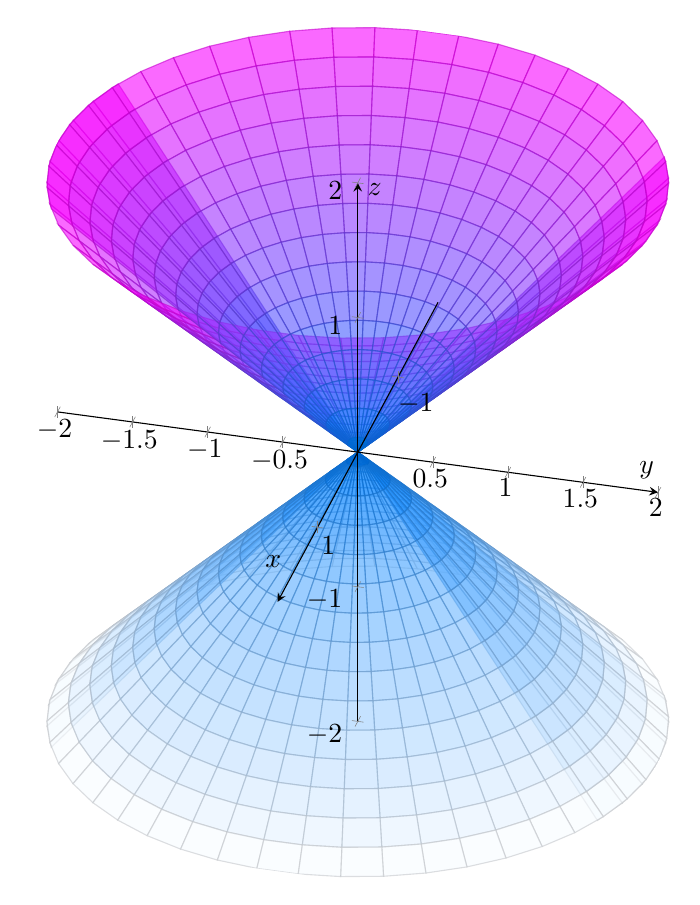
\begin{tikzpicture}
  \begin{axis}[
    view={105}{30},
    axis lines=center,
    axis equal image,
    xlabel={$x$},
    ylabel={$y$},
    zlabel={$z$},
    domain=-2:2,
    samples=30,
    colormap/cool,
    mesh/ordering=y varies,
    scale=3,
    axis on top,
  ]
  \addplot3 [surf,z buffer=sort,opacity=0.6] ({x*cos(deg(y))}, {x*sin(deg(y))}, {x});
  \addplot3 [surf,z buffer=sort,opacity=0.6] ({x*cos(deg(y))}, {x*sin(deg(y))}, {-x});
  \end{axis}
\end{tikzpicture}
\end{center}

\hfill

\noindent (b)
\begin{center}
    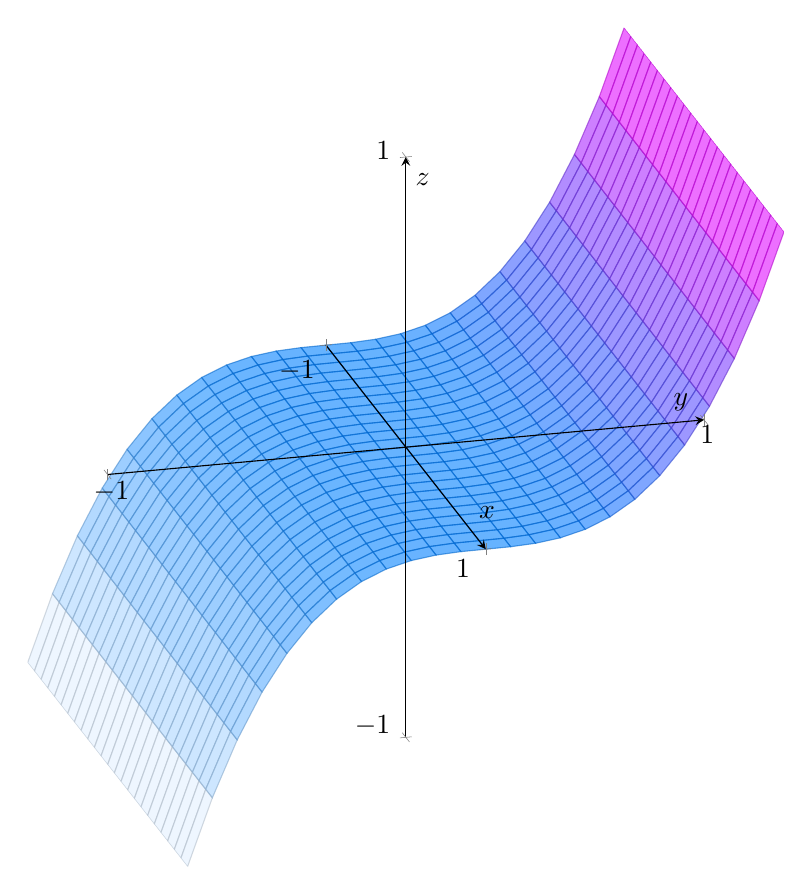
\begin{tikzpicture}
  \begin{axis}[
    view={75}{20},
    axis equal image,
    axis lines=center,
    xlabel={$x$},
    ylabel={$y$},
    zlabel={$z$},
    domain=-1:1,
    samples=25,
    colormap/cool,
    scale=2.2,
    axis on top,
    xtick={-1,1}, ytick={-1,1}, ztick={-1,1},
  ]
  \addplot3 [surf,z buffer=sort,opacity=0.6] {y^3};
  \end{axis}
\end{tikzpicture}
\end{center}

\newpage

\noindent 3. Find $\mathbf{R}(1)$.

\[\mathbf{R}(1)=\mathbf{i}-\mathbf{k}\]

\hfill

\noindent For $t=1$, we have the point $(1,0,-1)$ on the curve. The tangent vector of this curve is the first derivative of $\mathbf{R}$ with respect to the parametrization variable.

\begin{align*}\mathbf{T}=\frac{d\mathbf R}{dt}&=\left(\frac d{dt}\left(1+2\sin(2\pi t)\right)\right)\mathbf{i}+\left(\frac d{dt}\ln t\right)\mathbf{j}+\left(\frac d{dt}\cos(\pi t)\right)\mathbf{k}\\\\&=(4\pi\cos(2\pi t))\mathbf{i}+\left(\frac1t\right)\mathbf{j}+(-\pi\sin(\pi t))\mathbf{k}\end{align*}

\hfill

\noindent At $t=1$, the tangent vector is $\mathbf{T}(1)=\left(4\pi\right)\mathbf{i}+\mathbf{j}$. The parametric equations for a line that passes through the point $P_0(x_0,y_0,z_0)$ is given by
\[\left.\begin{array}{c}
x=x_0+T_1u\\
y=y_0+T_2u\\
z=z_0+T_3u
\end{array}\right\}\quad u\in\mathbb{R}\]

\hfill

\noindent Therefore, the equation of the line that is tangent to $C$ is

\[\boxed{\left.\begin{array}{l}
x=1+4\pi u\\
y=u\\
z=-1
\end{array}\right\}\quad u\in\mathbb{R}}\]

\hfill

\noindent 4. The value of the function at the point $(1,-2)$ is $4$. Therefore, we will show that the limit is also $4$. For every $\epsilon>0$, there exists a $\delta>0$ such that

\[0<\sqrt{(x-1)^2+(y+2)^2}<\delta\implies\left|f(x,y)-L\right|<\epsilon\]

\begin{align*}\left|\frac{4x^2-y}{2x+y}-4\right|&=\left|\frac{(2x-y)(2x+y)}{2x+y}-4\right|=\left|2x-y-4\right|=\left|2(x-1)+(-y-2)\right|\\\\&\leq2|x-1|+\left|-y-2\right|\quad \left(|a+b|\leq|a|+|b|\rightarrow\text{triangle inequality}\right)\\\\&=2|x-1|+|y+2|\end{align*}

\hfill

\noindent Since $\sqrt{(x-1)^2+(y+2)^2}<\delta\implies(x-1)^2+(y+2)^2<\delta^2$ and $(x-1)^2\geq0$ and $(y+2)^2\geq0$, we have $|x-1|\leq\delta$ and $|y+2|\leq\delta$.

\[2|x-1|+|y+2|\leq2\delta+\delta=3\delta\]

\hfill

\noindent Let $\delta=\dfrac\epsilon3$.

\[\left|\frac{4x^2-y}{2x+y}-4\right|\leq2|x-1|+|y+2|\leq3\cdot\frac\epsilon3=\epsilon\]

\hfill

\noindent Since the limit is equal to the value of the function at $(-1,2)$, $f$ is continuous at $(-1,2)$.

\hfill

\noindent 5. Apply the chain rule.

\[\frac{\partial w}{\partial u}=\frac{\partial w}{\partial x}\cdot\frac{\partial x}{\partial u}+\frac{\partial w}{\partial y}\cdot\frac{\partial y}{\partial u}+\frac{\partial w}{\partial z}\cdot\frac{\partial z}{\partial u}\]
\[\frac{\partial w}{\partial x}=\frac1z,\quad\frac{\partial w}{\partial y}=\frac{\cos y}z,\quad \frac{\partial w}{\partial z}=-\frac{x+\sin y}{z^2}\]
\[\frac{\partial x}{\partial u}=\frac1{u+v},\quad\frac{\partial y}{\partial u}=v\mathrm{e}^{uv},\quad\frac{\partial z}{\partial u}=-\frac1{u^2}\]

\begin{align*}\frac{\partial w}{\partial u}&=\frac1z\cdot\frac1{u+v}+\frac{\cos y}z\cdot v\mathrm{e}^{uv}+\frac{x+\sin y}{z^2}\cdot\frac1{u^2}\\\\&=\boxed{\frac u{u+v}+\mathrm{e}^{uv}uv\cos\left(\mathrm{e}^{uv}\right)+\ln(u+v)+\sin\left(\mathrm{e}^{uv}\right)}\end{align*}

\hfill

\noindent 6. The volume of a right triangular prism with opposite and adjacent sides and height $a=5,\:b=3,\:h=6$ is given by

\[V(a,b,h)=\frac12 abh\]

\hfill

\noindent For small errors, $\Delta V\approx dV$. The total differential of $V$ is

\[dV=V_ada+V_bdb+V_hdh\]

\hfill

\noindent Compute $V_a,\: V_b,\: V_c$.

\[V_a=\frac12bh=\frac12\cdot3\cdot6=9,\quad V_b=\frac12ah=\frac12\cdot5\cdot6=15,\quad V_h=\frac12ab=\frac12\cdot5\cdot3=\frac{15}2\]

\hfill

\noindent Given that $|da|\leq0.4,\:|db|\leq0.4,\:|dh|\leq0.4$. Calculate the bounds for the propagated error.

\[\left|dV\right|\leq9\cdot0.4+15\cdot0.4+\frac{15}2\cdot0.4=\boxed{\frac{63}5}\]

\hfill

\noindent 7. Let $g(x,y,z)=x^2+2y^2+z^2-1$ be the constraint. Solve the system of equations below.

\[
\left.
\begin{array}{c}
\displaystyle\nabla f=\lambda\nabla g\\
\displaystyle g(x,y,z)=0
\end{array}
\right\}\quad
\begin{array}{l}
\nabla f=\left\langle1,0,-1\right\rangle=\lambda\left\langle2x,4y,2z\right\rangle=\lambda\nabla g\\[1em]x=\dfrac1{2\lambda},\quad y=0\:\text{ or }\:\lambda=0,\quad z=-\dfrac1{2\lambda}
\end{array}
\]

\hfill

\[\lambda=0\implies x=y=z=0\implies f(0,0,0)=0\]

\[x=\frac1{2\lambda},\quad y=0,\quad z=-\frac1{2\lambda}\implies g\left(\frac1{2\lambda},0,-\frac1{2\lambda}\right)=\left(\frac1{2\lambda}\right)^2+2\cdot0^2+\left(-\frac1{2\lambda}\right)^2=1\]
\[\frac1{2\lambda^2}=1\implies\lambda=\pm\frac1{\sqrt2}\]

\hfill

\[\lambda=\frac1{\sqrt2}\implies x=\frac1{\sqrt2},\: y=0,\: z=-\frac1{\sqrt2}\qquad\lambda=-\frac1{\sqrt2}\implies x=-\frac1{\sqrt2},\: y=0,\: z=\frac1{\sqrt2}\]

\hfill

\[f\left(\frac1{\sqrt2},0,-\frac1{\sqrt2}\right)=\frac1{\sqrt2}+\frac1{\sqrt2}=\sqrt2\qquad f\left(-\frac1{\sqrt2},0,\frac1{\sqrt2}\right)=-\frac1{\sqrt2}-\frac1{\sqrt2}=-\sqrt2\]

\hfill

\noindent Compare the values $\displaystyle f(0,0,0),\:f\left(\frac1{\sqrt2},0,-\frac1{\sqrt2}\right),\:f\left(-\frac1{\sqrt2},0,\frac1{\sqrt2}\right)$.

\hfill

\[\boxed{\text{The minimum value is }{-\sqrt2},\text{ the maximum value is }\sqrt2.}\]

\hfill

\noindent 8. To identify the critical points, find where both $f_x=f_y=0$ or one of the partial derivatives does not exist.

\[f_x=3x^2+y,\quad f_y=-3y^2+x\]
\[\left.\begin{array}{c}
f_x=0\implies-y=3x^2\\
f_y=0\implies3y^2=x 
\end{array}\:\right\}\:-y=27y^4\implies y(27y^3+1)=0\implies y_1=0,\quad y_2=-\frac13\]

\[y_1=0\implies x_1=0,\quad y_2=-\frac13\implies x_2=\frac13\]

\hfill

\noindent The critical points are $(0,0)$ and $\left(\frac13,-\frac13\right)$. To classify these points, calculate the second partial derivatives and then find the Hessian determinants.

\[f_{xx}=6x,\quad f_{xy}=f_{yx}=1,\quad f_{yy}=-6y\]

\[(0,0)\rightarrow\left\{\:\begin{array}{l}
f_{xx}=0,\quad f_{xy}=1,\quad f_{yy}=0\\[1em]
\left|\begin{array}{cc}
0 & 1\\
1 & 0
\end{array}\right|=0\cdot0-1\cdot1=-1<0
\end{array}\right.\]

\[\left(\frac13,-\frac13\right)\rightarrow\left\{\:\begin{array}{l}
f_{xx}=2,\quad f_{xy}=1,\quad f_{yy}=2\\[1em]
\left|\begin{array}{cc}
2 & 1\\
1 & 2
\end{array}\right|=2\cdot2-1\cdot1=3>0,\quad f_{xx}>0
\end{array}\right.\]

\[\boxed{\text{A local minimum occurs at }\left(\frac13,-\frac13\right)\text{ and a saddle point occurs at }(0,0).}\]

\end{document}